\section{传质引论}
\subsection{概述}
\subsection{传质入门}
\subsubsection{传质速率定律}
\begin{itemize}
    \item 菲克扩散定律
    对于一维双组份扩散的情况:
    \begin{equation}\label{equ:fick_law_1d}
        \dot{m}_A'' = Y_A(\dot{m}_A'' + \dot{m}_B'') - \rho \mathcal{D}_\mathrm{AB}\frac{\dd Y_A}{\dd x}
    \end{equation}{\tiny 这里要特别注意,虽然\(\dot{m}_A'' + \dot{m}_B''=\dot{m}''\),但并不意味者\(Y_A \dot{m}''\)就等于\(\dot{m}_A''\)。因为当中还涉及到了扩散作用。}

    \textbf{质量通量}的定义为垂直于流动方向的单位面积质量流量:
    \begin{equation}
        \dot{m}_A'' = \dot{m}_A/A.
    \end{equation}

    可以写成更一般的形式:

    \begin{equation}
        \dot{m}_{\mathrm{A}}^{\prime\prime}=Y_{\mathrm{A}}\,(\dot{m}_{\mathrm{A}}^{\prime\prime}+\dot{m}_{\mathrm{B}}^{\prime\prime})-\rho D_{\mathrm{AB}}\nabla Y_{\mathrm{A}},
    \end{equation}
    \begin{equation}
        \dot{N}_{\mathrm{A}}^{\prime\prime}=\chi_{\mathrm{A}}(\dot{N}_{\mathrm{A}}^{\prime\prime}+\dot{N}_{\mathrm{B}}^{\prime\prime})-c D_{\mathrm{AB}}{\nabla}\chi_{\mathrm{A}},
    \end{equation}
    
    其中\(c\)是混合物的浓度(kmol/m\(^3\))。

    如果我们同时考虑A和B的扩散,将两个物质的式~\ref{equ:fick_law_1d}相加,可以得到:

    \begin{equation}
        -\rho\mathcal{D}_\mathrm{AB}\frac{\dd Y_A}{\dd x} - \rho\mathcal{D}_\mathrm{BA}\frac{\dd Y_B}{\dd x} = 0
    \end{equation}

    \item 扩散的分子基础
    扩散系数和温度及压强的关系:
    \begin{equation}
        \mathcal{D}_\mathrm{AB} \propto T^{3/2}P^{-1}
    \end{equation}

    而质量通量实质上是和\(\rho \mathcal{D}_\mathrm{AB}\)相关,它仅和温度相关:
    \begin{equation}
        \rho\mathcal{D}_\mathrm{AB}\propto T^{1/2}
    \end{equation}
    \item 与热传导的比较
\end{itemize}

\subsubsection{组分守恒}
考虑化学反应:
\begin{equation}
    \frac{\dd m_{\mathrm{A}, cv}}{\dd t} = [\dot{m}_A'' A]_x - [\dot{m}_A'' A]_{x+\Delta x} + \dot{m}_A''' V
\end{equation}

经过整理可以得到:
\begin{equation}
    \frac{\pp(\rho Y_A)}{\pp t} = -\frac{\pp}{\pp x}\left[Y_A\dot{m}'' - \rho \mathcal{D}_\mathrm{AB}\frac{\pp Y_A}{\pp x}\right] + \dot{m}_A'''
\end{equation}

对于稳态的情况:
\begin{equation}
    \dot{m}_A''' - \frac{\dd}{\dd x}\left[Y_A\dot{m}'' - \rho\mathcal{D}_\mathrm{AB}\frac{\dd Y_A}{\dd x}\right] = 0.
\end{equation}

把括号里面的东西打包的话其实也可以写作:
\begin{equation}
    \dot{m}_A''' - \nabla\cdot \dot{m}_A'' = 0
\end{equation}

\subsection{传质的应用实例}
\subsubsection{斯蒂芬问题}

% \begin{figure}[H]
%     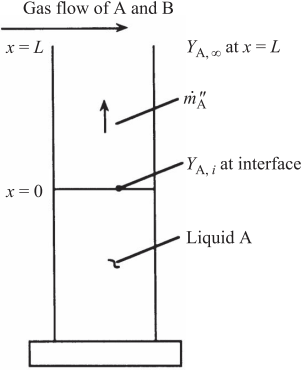
\includegraphics[width=.3\textwidth]{img/stefan.png}
% \end{figure}

我们考虑液体A在玻璃圆通内保持一个固定的高度,假设B在A中不可溶解,由此圆柱中存在着一个B的滞止层。对于这个问题,A的质量通量为:

{\tiny\begin{equation}
    \dot{m}''_A = \frac{\rho \mathcal{D}_\mathrm{AB}}{L}\ln\left(\frac{1-Y_{A,\infty}}{1-Y_{A,i}}\right)
\end{equation}
}
推导过程如下:
{\scriptsize\color{gray}

由于B的量通量为0,基于菲克定律式~\ref{equ:fick_law_1d},我们可以写出
\[
    \dot{m}_A'' = Y_A\dot{m}_A'' - \rho \mathcal{D}_\mathrm{AB}\frac{\dd Y_A}{\dd x}
\]对之整理并分离变量:
\[
    -{\frac{\dot{m}_{\mathrm{A}}^{\prime\prime}}{\rho D_{\mathrm{AB}}}}\mathrm{d}x={\frac{\mathrm{d}Y_{\mathrm{A}}}{1-Y_{\mathrm{A}}}}.
\]
积分解得:
\[
    -{\frac{\bar{m}_{\mathrm{A}}^{\prime\prime}}{\rho D_{\mathrm{AB}}}}\,x=-\ln[1-Y_{\mathrm{A}}]+C,
\]结合已知边界条件,\(Y_A(x=0)=Y_{A,i}, Y_A(x=L)=Y_{A,\infty}\)。}

就可以写出质量分数的计算公式:

\begin{equation}
    Y_A(x) = 1 - (1-Y_{A,i})\exp\left(\frac{\dot{m}_A'' x}{\rho\mathcal{D}_\mathrm{AB}}\right)
\end{equation}

\subsubsection{液-气界面的边界条件}

不难写出\(\chi_{A,i} = P_\mathrm{sat}/P\),由此可以确定质量分数应该为:
\begin{equation}
    Y_{A,i} = \frac{P_\mathrm{sat}(T_\mathrm{liq, i})}{P}\frac{\mathrm{MW}}{\mathrm{MW}_\mathrm{mix, i}}
\end{equation}

认为液-气界面上维持温度的连续性,那么:
\[
    T_\mathrm{liq,i}(x=0^-) = T_\mathrm{vap, i}(x=0^+) = T(0)
\]


\subsubsection{液滴蒸发}

\textbf{假设}:
{\scriptsize
    \begin{enumerate}
        \item 蒸发过程是准稳态的。
        \item 液滴的温度均一,进而假设温度为低于液体的沸点的某一定值。
        \item 液滴表面蒸气的质量分数由液滴温度下的液体-蒸气平衡确定。
        \item 假设所有的热物理参数——特别是\(\rho\mathcal{D}\)——是常数。
    \end{enumerate}
}

\textbf{蒸发速率}:

从某种意义上说,这里的液滴蒸发问题其实就是一个加强版的球状的斯蒂芬流。定义\textbf{传质数}\(B_Y\)为:
\begin{equation}
    B_Y = \frac{Y_{A,s}-Y_{A,\infty}}{1 - Y_{A,s}}
\end{equation}
蒸发速率可以被写作:
\begin{equation}\label{equ:evo_rate}
    \dot{m}_A''' = {4\pi r_s \rho \mathcal{D}_\mathrm{AB}}\ln({1+B_Y})
\end{equation}

具体的推倒过程如下所示:

{
    \scriptsize\color{gray}
    首先,液滴的蒸发速率可以被写作
    \[
        \dot{m}(r) = 4\pi r^2 \dot{m}''
    \]
    将之带入到菲克定律~\ref{equ:fick_law_1d}的表达式中,并且认为另一组份滞止,可以得到:
    \[
        \dot{m}_A'' = Y_A\dot{m}_A'' - \rho\mathcal{D}_\mathrm{AB}\frac{\dd Y_A}{\dd r}
    \]
    代入蒸发速率的表达式,并且整理,可以得到:
    \[
        \dot{m}=-4\pi r^2 \frac{\rho \mathcal{D}_\mathrm{AB}}{1-Y_A}\frac{\dd Y_A}{\dd r}
    \]
    首先代入液滴表面的边界条件\(Y_A(r=r_s)=Y_{A,s}\),可以得到:
    \[
        Y_{\mathrm{A}}(r)=1-{\frac{(1-Y_{\mathrm{A,s}})\exp[-\dot{m}/(4\pi\rho \mathcal{D}_{\mathrm{AB}}r)]}{\exp[-\dot{m}/(4\pi\rho \mathcal{D}_{\mathrm{AB}}r_{s})]}}.
    \]
    再代入\(r\to\infty\)时,\(Y_A=Y_{A,\infty}\),可以解得蒸发速率\(\dot{m}\)的最终结果。
}

\textbf{液滴质量守恒}:

显然,液滴质量和蒸发速率之间的关系是:

\begin{equation}
    \frac{\dd m_d}{\dd t}=-\dot{m}
\end{equation}
液滴的质量可以写作:
\begin{equation}
    m_d = \rho_l V = \rho_l \pi D^3/6
\end{equation}
将这两个式子代入到液滴蒸发速率的公式中(式~\ref{equ:evo_rate}),化简唯粉整理,可以得到:
\begin{equation}
    \frac{\mathrm{d}D}{\mathrm{d}t}=-\frac{4\rho \mathcal{D}_\mathrm{AB}}{\rho_{i}D}\mathrm{ln}(1+B_{Y}).
\end{equation}
或者是:
\begin{equation}\label{equ:03_evap}
    {\frac{\mathrm{d}D^{2}}{\mathrm{d}t}}=-{\frac{8\rho \mathcal{D}_{\mathrm{AB}}}{\rho_{l}}}\ln(1+B_{Y}).
\end{equation}

我们将等式的右边定义为\textbf{蒸发常数}:
\begin{equation}
    K = {\frac{8\rho \mathcal{D}_{\mathrm{AB}}}{\rho_{l}}}\ln(1+B_{Y})
\end{equation}

由此可以得到\(D\)随时间\(t\)的关系式:
\begin{equation}
    D^2(t)=D_0^2 - Kt
\end{equation}
这就是\textbf{\(D^2\)定律}。

\begin{figure}[H]
    \centering
    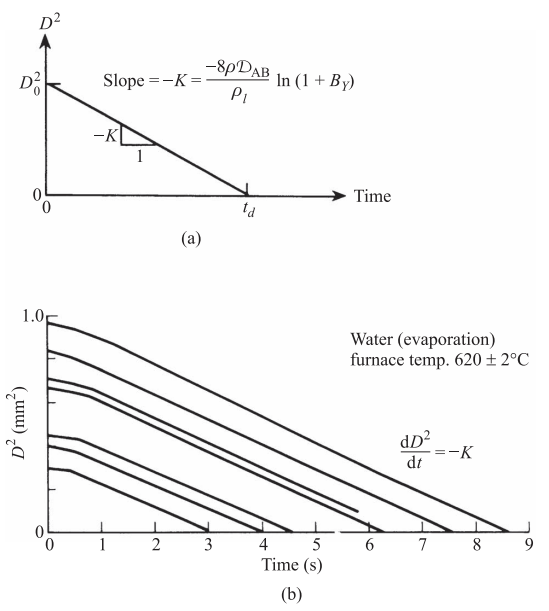
\includegraphics[width=.3\textwidth]{img/d2.png}
\end{figure}
